\newif\ifhandout %create boolean variable handout

\handouttrue %set handout to false

\ifhandout %test if we want to create handout or slides
	\documentclass[handout]{beamer}
	\usepackage{pgfpages}
	\pgfpagesuselayout{4 on 1}[a4paper,border shrink=5mm]
\else 
	\documentclass{beamer}	
\fi

\usepackage[utf8]{inputenc} % Charakter-Kodierung
\usepackage[german]{babel} % Sprache

%\usepackage[table,xcdraw]{xcolor} % Tabellen Farben
\usepackage{tabularx} % Dynamische Tabellenbreite
\usepackage{tcolorbox} % Graue Boxen
\usepackage{hyperref} % url Umgebung
\usepackage{natbib} % Bibliographie
\usepackage{fancyhdr} % Header und Footer
\usepackage{multirow} % Multizeile
\usepackage{geometry} % Page layout
%\usepackage{color} % Text Farben
\usepackage{longtable} % lange Tabelle

% Bibstyle
%\bibliographystyle{plain}
%\bibliography{bib/master.bib}

%\setbeamertemplate{footline}[frame number]

\setbeamertemplate{footline}{
	\hfill
	\insertframenumber /\inserttotalframenumber
	\hrule
}
\setbeamertemplate{headline}{
%\includegraphics[width=4cm]{img/cau-logo-2017}
\hfill%
%\includegraphics[width=1cm]{img/se-logo}
\hrule
}
\addtobeamertemplate{background canvas}{\transfade}
% Titelseite

\title{
	Einfluss der Datenbasis\\
	\color{gray}
	Bennet Bleßmann\\
}

\date{\today}


% Dokument

\begin{document}
	\begin{frame}	
\titlepage
\end{frame}
	\mode<beamer>{	
		\frame{\frametitle{Inhaltsverzeichnis}\tableofcontents}
	}
	\section{Einführung} 
\begin{frame}
\frametitle{Einführung}
\framesubtitle{Was ist die Datenbasis?}
\setbeamercovered{transparent}
\end{frame}
	\section{Problems}

\subsection{Requirements Phase}
Problems not being acknowledged in this phase might be hard to resolve at a later stage as this phase presents the foundation for all further phases. 

\subsubsection{Vague Goal}
%explanaition
For example an unspecified fairness metric would be a vague goal for a selection algorithm that could result in an algorithm to be considered unfair.
%example
Another example might be to have the goal to increase one's profit. This may be achieved by increasing efficiency to expand the profit margin on the product, or by implementing better advertisement strategies to get more buying consumers. Both would be valid strategies but, depending on the circumstances, either might be preferred over the other and each entails other possible problems. Therefore the goal to increase profit is vague as it is unclear which option is wanted.  

\subsubsection{Moral Acceptability}

%explanaition
Another less concrete problem is the consideration whether an algorithms should be developed at all in the sense that an algorithm can be technically possible but morally unwanted.

%example 
As an example:
I have no doubt that it is possible to develop better filters for the Great Firewall of China, but from a humanitarian standpoint I would disagree to build such.

\subsubsection{Economic Incentive}

%explanation
Probably the most tangible problem is the collision of morality and ethics with economics. 
In most circumstances, in  the current economic structure, it would be unreasonable to produce an algorithm without any direct economic benefit, even if it would be socially beneficial. 
On the other hand it might be of interest to produce an ethically, morally or socially problematic algorithm for one's economical benefit. 

%example
For example:
One could consider writing filters for China due to an economic benefit offered by the government.

\subsection{Planning Phase}
Since this is the phase in which we expect most decisions to be made and 
the most information to become available, this is also a rather important phase.

\subsubsection{Incorrect/Insufficient Model}
%explanation

A model might be insufficient by representing reality oversimplified or overcomplicated.

%example
For example the chatbot that had been deployed by Microsoft
 which turned into "[..] a racist asshole in less than a day" (\cite{James2018} was oversimplified, missing the difference between acceptable and unacceptable tweets.
 
\subsubsection{Insufficient Safety Considerations}
%explanation
This problem includes unconsidered IT security or data protection risks, as well as, where applicable, risk to the physical world.
External threats are usually sufficiently covered, while internal threats are sometimes forgotten or not sufficiently treated. 

\subsection{Implementation Phase}
This phase is basically identical to your typical implementation 
phase and therefore the same problems apply.

\subsubsection{Missing Documentation}
% Mangelnde Dokumentation (Annahmen, Funktionsweise etc.)

Missing documentation is mostly a problem in the case of undocumented assumptions which might result in unmet requirements and consequently in undefined behaviour. For example, if a function assumes inputs to be sanitised without this being documented, unsanitized data might be passed to it and lead to unwanted behaviour. Documentation can also help when maintaining a deployed product, which is part of a phase described later.

\subsection{Training Phase}
This is the last phase before the algorithm goes into production and also the one where the problems might be hard to predict, observe directly and diverge most from traditional programming. The focus will be on the data used for training rather than on the training itself.

\subsubsection{Restricted Representation of Reality}
% Unzureichende Abbildung der Realitzät durch Trainingsdaten

Training data is insufficient representative when it diverges from reality in essential parts. This can be seen at the example of election predictions (\cite{2016}) in the difference between the prediction and the result, where the difference is sometimes significant.

\subsubsection{Incorrect Information}
% Unreine Daten

Incorrect information might be misspelled names, mislabelled images et cetera. For example a misplaced comma in a report to a credit scoring firm might ruin one's credit score which has the potential to ruin a life.

\subsubsection{Irrelevant Information}
% Irrelevante Daten
%alg shall be used in amarica trained on world wide data

Irrelevant data is present when the data contains 
objects which are not supposed to be in the production 
environment. This does not mean the data is incorrect,
for example an algorithm only to be deployed to evaluate
Irish consumers that is also trained with data from 
Belgian consumers would fall into this category.
The problem is that in this example the algorithm
would have to handle more varied inputs with the same resources, resulting
in worse performance.

\subsubsection{Contaminated Data}
% Korrekte aber unpassende Daten (wiederspiegeln von Rassismus in der Gesselschaft etc.)

Additionally to the already mentioned cases, data can be problematic 
in at least one other way, as even correct, clean, truthfully representing data might not result in what was intended.
This can best be seen in the example of Amazon's employment evaluation algorithm (\cite{Higginbottom2018}). It was given the data of the currently employed workforce and was suppose to evaluate if applicants would be a good addition.
Since the workforce was dominantly male it was biased against females.

\subsection{Deployment/Maintenance Phase}
This phase mostly consists of problems inherent to
deep-learning algorithms. As such they are hardly 
able to be avoided.

\subsubsection{Lack of Traceability}
% Fehlende Nachvollziehbarkeit

In opposition to traditional algorithms, most deep-learning-algorithms are not comprehensible, as they are a set of numbers, computed based on some training data and an initial configuration, with no further justification, explanation or reason. In traditional algorithms an anomaly can usually be traced back to either an error in human intuition, meaning the result is correct even if this is not obvious, or an error in the algorithm which can than be resolved through correction. 

\subsubsection{Unforeseen Influences and Consequences}
% Unvorhergesehene Einflüsse

Unforeseen influences and consequences mostly come in pairs because one is usually the result of the other. For example it has been demonstrated (\cite{Eykholt2017})that it is possible to modify street signs in a way that an image classification algorithm misclassified street signs with high confidence, while being still legible from a human perspective.
%(Payed Positive Reviews -> Useless Reviews)

\subsubsection{Liability and Legal Responsibility}
% Unklare Haftung (Nutzer, Produzent, Entwickler ?)

As with all automated decision making processes 
it is not in all circumstances clear who is liable for 
the decisions made and has to take responsibility.
The example most talked about would probably be 
that of autonomous vehicles. Usually, either the driver or the manufacturer would be to blame for an accident, depending on the cause. In case of autonomous vehicles the car would be the main source of failure. This could cause a liability problem for manufacturers.   
Depending on the level of autonomy and the manufacturer complying with due diligence it might even be the case that neither the manufacturer nor the owner should be responsible. Which might pose a problem to the legal system, especially where a party exists that normally would have received compensation from the responsible party.

	\section{Solutions}
In this section I will present possible solution
for the individual problems where possible.

\subsection{Vague Goals}
When a vague goal is encountered the best option is to reiterate this goal with the entity that has set this goal an let them specify what they meant. For our example where the options to increase profitability where better advertisement or finding inefficiencies and removing them, these options could than be presented to the client so they can decide which to pursue.


\subsection{Moral Acceptability}
If the problem would be that the algorithm could be misused
this might be fixable, as one could try to eliminate or limit this possibility to a satisfiable degree.

\subsection{Economic Incentive}
Depending on the algorithm the government can
give incentives to reduce the financial load
to produce algorithms beneficial to the public and
produce laws limiting the extend of e.g. privacy invading algorithms.

%%%%%%%%%%%%%%%%%%%%%%%%%%%%%%%%%%%%%

%\subsection{Incorrect/Insufficient Model}
%\subsection{Insufficient Safety Considerations}

%%%%%%%%%%%%%%%%%%%%%%%%%%%%%%%%%%%%%

\subsection{Missing Documentation}
To reduce the amount of missing documentation
one can use tools like for example linters to warn if 
functions are undocumented. Also one can write documentation 
first before writing the code similar to test driven development.

%\subsection{Missing Data Protection}


%%%%%%%%%%%%%%%%%%%%%%%%%%%%%%%%%%%%%

\subsection{Insufficient Representation of Reality}
There will in most cases be asymmetries between the production
and testing environment, but reducing these should help with 
this issue for example when training a chatbot if your production environment doesn't filter the messages your testing
environment shouldn't filter as well, that way the bot 
learns how to react messages that would have been filtered, on the other hand  if only the testing environment would be filtered, how the bot responds messages that would have been filtered in testing
is basically undefined behaviour.

\subsection{Dirty Data}
The amount of dirty data can be reduced by limiting 
the amount of manual data entry as this is types of errors 
are usually caused by human error. This is not to say that other sources are
always correct optical character recognition also known as OCR can 
also misidentify characters and cause similar problems.
Where available comparing different sources may also be employed to detect errors.

%Irrelevant data

%contaminated data

%%%%%%%%%%%%%%%%%%%%%%%%%%%%%%%%%%%%%

%lack of traceability  ¯\_(ツ)_/¯
%Unforseen Influences and Consequences
%Liability and Legal Responsibility







	\section{Ethik}
\begin{frame}
\frametitle{Ethik}
%TODO
\end{frame}
	\section{Diskussion}
\begin{frame}
\frametitle{Diskussion}
\setbeamercovered{transparent}

\end{frame}

\begin{frame}
\frametitle{Diskussion}
\setbeamercovered{transparent}

\end{frame}

\begin{frame}
\frametitle{Diskussion}
\setbeamercovered{transparent}

\end{frame}
	\section*{Quellen}
\begin{frame}
\frametitle{References}
%\nocite{*}
%\printbibliography
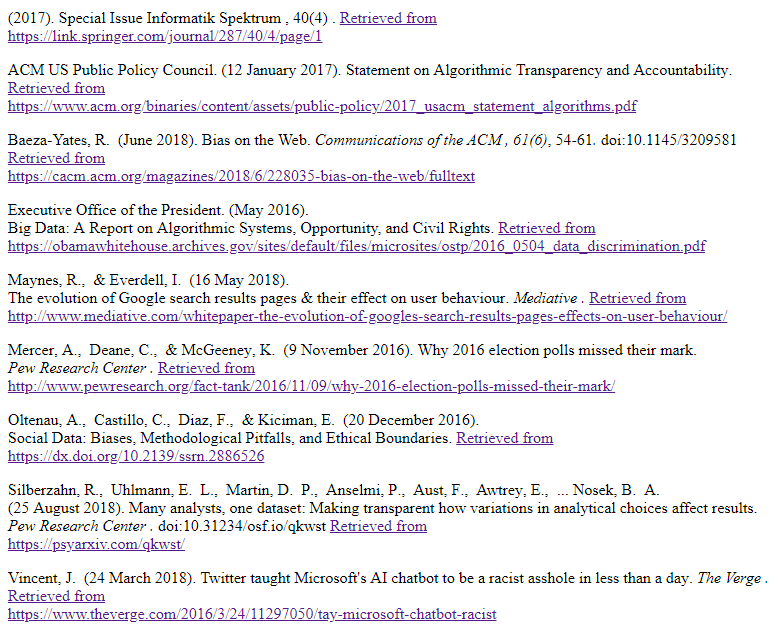
\includegraphics[width=\textwidth]{img/ref}
\end{frame}

\section*{Danke}
\only<beamer:1|handout:0>{
\begin{frame}
\frametitle{Vielen Dank}
Vielen Dank fürs Zuhören und Teilnehmen
\end{frame}
}
\end{document}